\documentclass[10pt,a4paper]{article}
\usepackage[utf8]{inputenc}
\usepackage{url}
\usepackage[english]{babel}
\usepackage{amsmath}
\usepackage{amsfonts}
\usepackage{amssymb}
 \usepackage{float}
\usepackage{graphicx}
\usepackage[left=2cm,right=2cm,top=2cm,bottom=2cm]{geometry}
\author{Andres Chaves}
\title{Report 3: Problem Definition and Expected Results}

\begin{document}
 \title{Report 3: Problem Definition and Expected Results}
 \author{Andres Chaves (706801) \\
  \multicolumn{1}{p{.7\textwidth}}{\centering{achaves@student.unimelb.edu.au\\}\centering\emph{Melbourne School of Information\\The University of Melbourne}}}
 \maketitle


 \begin{abstract}
    The purpose of this document is to refine the problem definition, based on the data exploration we made and the reports written through this research project, and also state the expected results of the project.
\end{abstract}

 \section*{Introduction}
Several reports have been written, as part of this research project. The research proposal was the foundation of this research, establishing the draft of the purpose, objectives and results.
\\\\
The first report attempted to further describe the problem by giving an overall of SNMP, Network Management, the particular network from which we have collected the alarm data and the data itself. In that report, we also performed some data exploration and correlation scenarios based on a probabilistic hypothesis.
\\\\
The second report analysed further the scenarios described in report 1 by the construction of a Bayesian Belief Network and also proposed some further scenarios.
\\\\
In this report we will formalise the problem statement and also describe the expected results

 \section{Background}
 There is no doubt on the strong development and evolution of information technologies in the modern world. Nowadays, we have access to computing devices in several forms such as supercomputers, laptops, tablets and smart phones; and of course this device evolution comes in conjunction with advances in distributed information systems.
 \\\\
 But this evolution could not be accomplished without a key component: computer networks. Networks allow data exchange and information services consumption possible and side by side with information technology, they have evolved from simple small low bandwidth networks to high speed wired and wireless ones connecting all the world. Several factors such as, the increase in size, support for different services and technologies and heterogeneity of vendors augments the complexity of networks\cite{autonomicComputing}.

 \subsection{Network Management}
 These complex networks require a set of practices, tools and knowledge in order to guarantee the availability and quality of service required by clients. A discipline called Network Management has arisen to address all these concerns and nowadays Network Management comprises all the practices and activities that a carrier must perform in order to fulfil its Service Level Agreements (SLAs) with its clients\cite{networkMgmtFund}.
 \\\\
 From the information systems perspective, Network Management requires a set of systems called Network Management Systems (NMS), designed to administer either all or a part of the network. This administration is composed by a set of functions: Fault Management, Performance Management, Configuration Management and Security Management among others\cite{ITU3010}.
 \\\\
The ITU-T proposes a layered Network Management System architecture. Figure \ref{fig:ITULayerArchitecture} illustrate the proposed layers. The description of each layer is as follows\cite{ITU3010}: 

\begin{itemize}
\item Network Element Layer, composed by the network elements itself. They interact with the next layer in a synchronous request/response way or asynchronously by sending alarms.
\item Element Management Layer, composed by Element Management Systems (EMS), which are systems designed to manage a segment or part of the network.
\item Network Management Layer, composed by Network Management Systems and Fault Management Systems allow the administration of a network as a whole.
\item Service Layer, allows a service oriented vision of the network.
\item Business Layer, which converts network and services into relevant business elements.
\end{itemize}

 \begin{figure}[H]
 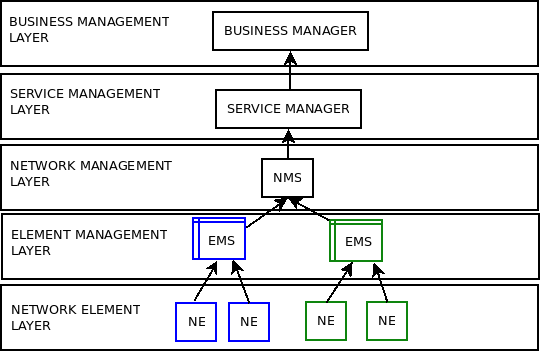
\includegraphics[scale=0.5]{ITU-Layered.png}
  \centering
  \caption{\textit{A diagram of the ITU-T proposed architecture}}
  \label{fig:ITULayerArchitecture}
\end{figure}	

It can be seen from the architecture that the the higher the layer, the higher the level of abstraction of the managed concepts. Subsequently, the lower the layer the higher the level of detail. It is important to say also, that the EMS systems receive and manage all the alarms of the subnetwork, whereas the NMS receive only the relevant alarms from the different EMS.

 \subsection{Fault Management}
 Fault Management involves how to detect, classify and inform network operators about conditions that affect or may affect the network services, both from availability and performance perspective. Accurate and timely fault detection allows the minimisation of the Mean Time To Detect (MTTD) and Mean Time To Repair (MTTR), increasing Network Availability. Typically, network elements inform this to an  information system, which can be part of an EMS or NMS, in an asynchronous way using SNMP protocol, specifically a SNMP TRAP event\cite{snmp}.
\\\\
One of the main approachs to detect failure is by monitoring the alarms received from the different network elements. These alarms are received in the EMS or FMS, according to the abstraction level. A FMS can be seen as a pipeline system that receives the alarm, translates it, enrich it with information from other sources and present it to the network operator.


 \section{The Challenge of Fault Management}
 One of the challenges in Network Management is how to monitor ever bigger networks where there are network devices in the range of thousands to millions. With a network of this size, the rate of alarms received by a system can be around hundreds of events per second and with this alarm ratio a key desired function of a FMS is to only show the relevant alarms to the network operators.
 \\\\
The increase in the number of alarms is due to several reasons, firstly we have the inherent growing of the network. Secondly, the same underlying event or failure can be seen from different network elements and each of them report it separately to the FMS. Thirdly, some network elements are designed to send an event alarm constantly. Lastly, we have heterogeneity of network elements, where the implementation of protocols or drafts vary between different vendors and subsequently generate diverse alarms when interoperate with each others\cite{ruleDiscoveringInNM}.
 \\\\
The challenge consist on how to handle the volume of alarms and how to display to the network operator the most representative alarms that encapsulate the cause and not the symptoms\cite{ruleDiscoveringInNM}.
 \\\\
To cope with this alarm volume and to display only relevant key alarms that reflects the failure events, the ITU recommends a correlation component based on rules, topology or expert systems and this is the approach taken by many commercial tools in the market. \cite{ITU3010}
 \\\\
All this correlation approaches are complementary between each other and have advantages and disadvantages. Typically, the expert systems are built by the same network element vendor, which guarantees correctness and efficiency of it. Sadly, those system only are only applicable in a given subdomain/vendor. 
\\\\
Topology correlation simplifies the network elements relations in a parent/child tree, and suppress alarms from the descendants whenever an alarm in a node occurs. The issue with this is that a topology must be updated for all the changes in the network.
\\\\
Finally, the rule based correlation requires a domain expert to write the rules. This desired expert is a person who knows about networking, the concrete network, the specific vendors and the relation between events and alarms. Normally it is difficult to find such an expert or he/she may not have enough time to spend in the correlation rules writing.
 
 \section{Problem Definition}

 One possible approach to analyse, classify and display only the relevant events to the operator is by the use of a machine learning system that helps the network operator to pre-process events and thus augment the network management capacity with the same engineering team size.
 \\\\
As we see in the challenge section, finding an expert to write the correlation rules may be difficult or not feasible. We propose an exploration about how Machine Learning techniques can be applied to aid the engineers in correlation rules discovering. If a system can infer or help to infer the rules, either the expert will generate the rules faster or an engineer with less expertise can accomplish the job.
 \\\\
 An alarm can be seen as a tuple of attributes $A=\{attr_1, atrr_2, attr_3, attr_4, attr_5\}$. The attributes of the alarms are:

\begin{itemize}
  \item Id: Unique numeric identifier of each alarm.
  \item Eventname: Correspond to the alarm name.
  \item Traptime: Timestamp of arrival of the alarm.
  \item Hostname: Ip or host name of the entity that sends the alarm.
  \item Formatline: Semi-structured formatted line of the alarm. Normally it includes all the alarm's bindings.
\end{itemize}

 The FMS has an historic of alarms, that is a set $S$ of alarms $S=\{A_1, A_2, ...,A_n\}$. This set can be ordered by traptime or id if required. An ideal system should take this set, analyse it and infer a set of rules.
 \\\\
But such an ideal system is not feasible due to the complexity of the search space. In order to develop an approximation of this desired system a heuristic, assumption or division of the problem must be done. In this sense we propose to divide the problem by selecting an alarm of interest and then infer the rules concerning to this alarm of interest. To further constrain the search space we propose to analyse the alarm of interest with the alarms encountered within a time window.
 \\\\
By selecting the alarm of interest $A_t$ and constrain the time window we can generate subsets $S_1, S_2, .., S_n\ where\ S_i \subset S$, $A_t \in S_i$ and the size of $S_i$ is constrained by the given time window. The machine learning algorithm can then take this subsets  as the training set and generate a set of correlation rules.


 \section{Evaluation of Results}

Given the constrained search space the solution should output either a set of rules or a degree of correlation between the different alarms in the input feature set.
\\\\
Each rule should have a degree of confidence and support and this two measurements can be used to guide the expert in the rule selection. It is expected that the generated rules are as general as possible.
\\\\
From a business perspective the rules might be evaluated by measuring what is the percentage of alarm suppressed. 
\\\\
Informally we want to have the following the results from the research project:
\begin{itemize}
\item Prove that Machine Learning can be applied in Fault Managament, specifically in network correlation rules generation
\item Illustrate that machine learning can help engineers to understand complex data
\item Illustrate that the generated rules "make sense" according to an expert criteria
\item Illustrate that the the implementation of the rules will suppress a great percentage of alarms
\item Propose further work on the subject
\end{itemize}


 \begin{thebibliography}{9}
\bibitem{autonomicComputing} Roy Sterrit,
        \emph{Towards Autonomic Computing: Effective Event Management}.
        SEW '02 Proceedings of the 27th Annual NASA Goddard Software Engineering Workshop (SEW-27'02), Page 40. ISBN: 0-7695-1855-9.
\bibitem{networkMgmtFund} Alexander Clemm,
        \emph{Network Management Fundamentals}.
       Cisco Press. ISBN-13: 978-1-58720-137-0.
\bibitem{ITU3010}\emph{ITU-T Recommendations, M.3010 principles for a
telecommunications management network}, Feb. 2000.
\bibitem{snmp}IETF RFC 1157, \url{http://www.ietf.org/rfc/rfc1157.txt?number=1157}.
\bibitem{ruleDiscoveringInNM} Roy Sterrit,
        \emph{Discovering Rules for Fault Management}.
 \end{thebibliography}
\end{document}